A series of tests were conducted to evaluate the effectiveness and accuracy of our approach. They were performed using different smartphones to verify the application's behavior with various Android versions and hardware resources, ensuring its compatibility and proper functioning. The tests consisted in using the application while walking along the instrumented path (in both directions), simulating real usage scenarios. The smartphone must be positioned in parallel to the floor, to ensure that QR codes placed on the floor can be properly framed and scanned. On the other hand, if the user intends to search for a specific point of interest through a QR code located on a door, the smartphone should be held in a vertical position. Figure \ref{fig:application-test} illustrates an example of the test procedure with the correct positioning of the phone.

\begin{figure}[H]
    \centering
    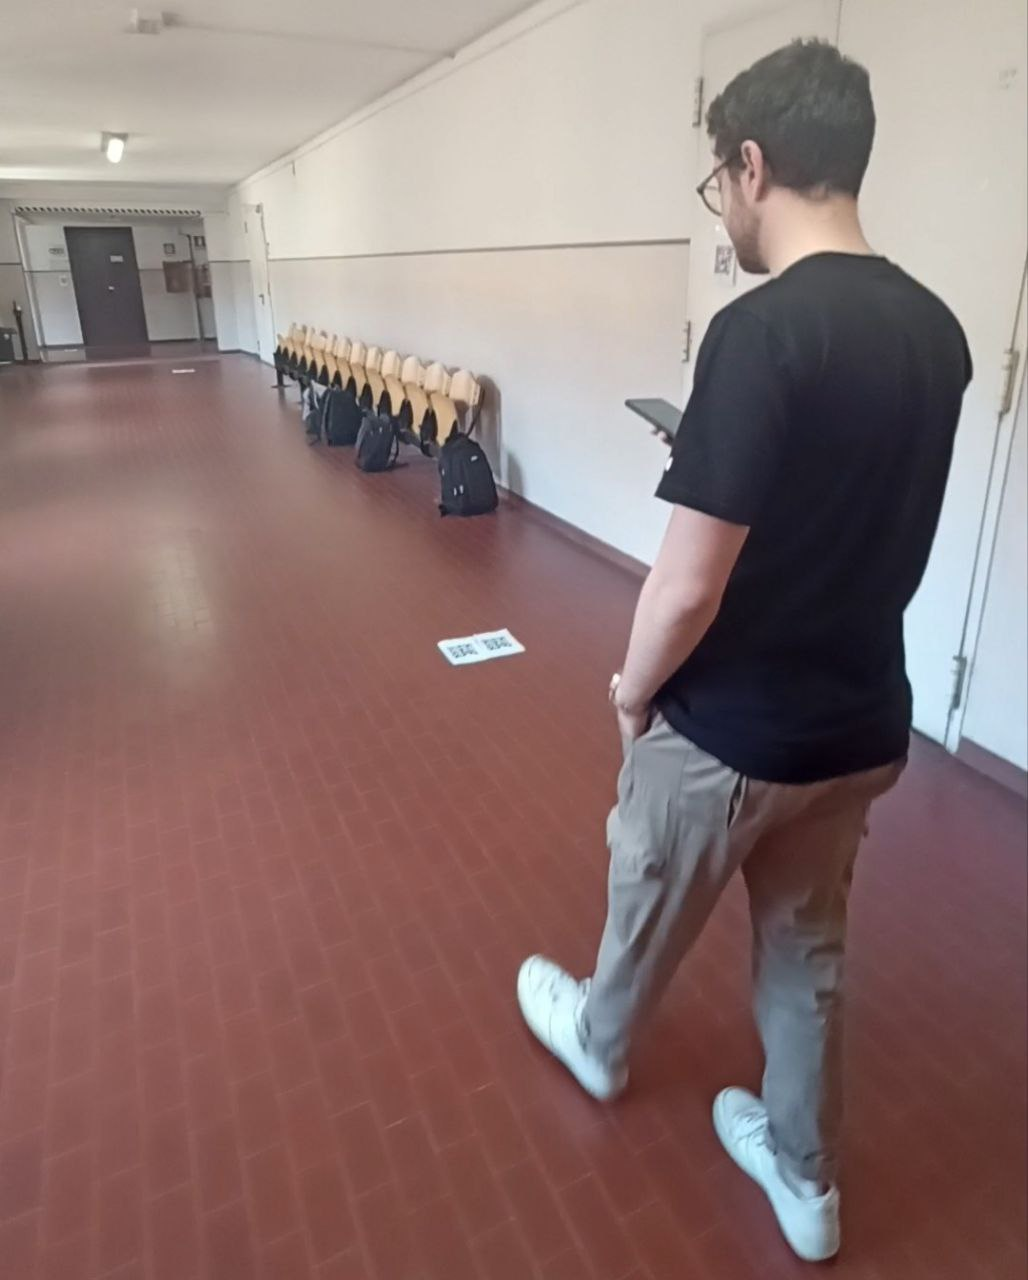
\includegraphics[width=0.8\columnwidth]{chapters/experimental_results/images/application_test.jpg}
    \caption{Final application tests}
    \label{fig:application-test}
\end{figure}

\subsubsection{Region change detection}
The evaluation focused on the application's ability to accurately detect transitions from one region to another. The application demonstrated the correct detection of region changes, with only sporadic instances of slight delay due to interference. In the majority of cases, the identification of new regions was performed accurately. The appropriate list of points of interest was provided to the users via the \textbf{TextToSpeech} \cite{android:text-to-speech-ref} functionality.

\subsubsection{Curve detection}
During the tests, we approached the curves along the path, and the application was evaluated on its capability to identify them and their direction (based on the previous region, which is always a pre-curve),  notifying users promptly. 
In most cases, the application demonstrated satisfactory performance in notifying users about curves, contributing to a smoother navigation experience.

\subsubsection{QR code detection}
The evaluation assessed the detection of QR codes placed on the ground and on the doors of points of interest. The application consistently and reliably detected floor QR codes while participants were walking, enabling the immediate delivery of audible notifications regarding nearby points of interest. Moreover, participants successfully scanned door QR codes, which allowed them to accurately determine the precise location of the points of interest.

\subsubsection{Application accessibility}
The conducted tests confirmed the application's compatibility with \textbf{Talkback} \cite{android:accessibility}, enabling visually impaired users to interact effectively with the application. 
These tests specifically focused on the different scenarios where user interaction is required. 

Additionally, \textbf{TextToSpeech} \cite{android:text-to-speech-ref} functionalities provide spoken announcements and instructions, eliminating the need for visually impaired users to rely on visual cues. In this way, visually impaired users will be able to use the application with ease.
